\documentclass[default]{beamer}
\setbeamertemplate{navigation symbols}{}

\usetheme{CambridgeUS}
\useoutertheme{infolines}
%\usecolortheme{crane}

\usepackage{cmap}							% Поддержка поиска русских слов в PDF (pdflatex)
\usepackage[T2A]{fontenc}       			%поддержка кириллицы
\usepackage[utf8]{inputenc}					% Выбор языка и кодировки
\usepackage[english, russian]{babel}
\usepackage{csquotes}
\usepackage{tikz}
\usetikzlibrary{calc}
\usepackage{animate}
\usepackage{fp}

\usepackage[
	language=auto,
	autolang=other,
	backend=biber,
	style=authortitle,
	sorting=ydnt
]{biblatex}
\addbibresource{common-cog.bib}
				
\DeclareSourcemap{
	\maps[datatype=bibtex, overwrite]{
		\map{
			\step[fieldset=langid, fieldvalue=english]
			\step[fieldset=doi, null]
			\step[fieldset=issn, null]
			\step[fieldset=isbn, null]
			\step[fieldset=url, null]
			\step[fieldsource=language, fieldset=langid, origfieldval]
		}
	}
}


\graphicspath{{../../images/}} 			% Пути к изображениям

\makeatletter
\setbeamertemplate{footline}
{
	\leavevmode%
	\hbox{%
		\begin{beamercolorbox}[wd=.333333\paperwidth,ht=2.25ex,dp=1ex,center]{author
				in head/foot}%
			\usebeamerfont{author in
				head/foot}\insertshortauthor~~\beamer@ifempty{\insertshortinstitute}{}{(\insertshortinstitute)}
		\end{beamercolorbox}%
		\begin{beamercolorbox}[wd=.333333\paperwidth,ht=2.25ex,dp=1ex,center]{title in
				head/foot}%
			\usebeamerfont{title in head/foot}\insertshorttitle
		\end{beamercolorbox}%
		\begin{beamercolorbox}[wd=.333333\paperwidth,ht=2.25ex,dp=1ex,right]{date in
				head/foot}%
			\usebeamerfont{date in head/foot}\insertshortdate{}\hspace*{2em}
			\insertframenumber{}\hspace*{2ex} 
		\end{beamercolorbox}
	}%
	\vskip0pt%
}


\renewcommand*{\bibfont}{\footnotesize}

\begin{document}
	
	\title[Знаковая картина мира]{Знаковая картина мира субъекта деятельности}
	\author[Панов]{Александр Панов}
	\institute[ФИЦ ИУ РАН]{Федеральный исследовательский центр <<Информатика и управление>>\\Российской академии наук}
	\date{25 апреля 2016~г.} 
	
	\begin{frame}
		\titlepage
	\end{frame}

	\begin{frame}
		\frametitle{Знаковая модель представления знаний}
		\small
		Компонентом представления знаний является знак:
		\begin{itemize}
			\item в смысле культурно-исторического подхода Выготского-Лурии,
			\item следуя теории деятельности Леонтьева.
		\end{itemize}
		
		\begin{columns}
			\begin{column}{0.4\textwidth}
				\centering
				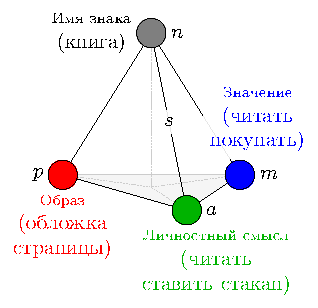
\includegraphics[width=\textwidth]{signs/sign_color_book_ru}
			\end{column}
			\begin{column}{0.6\textwidth}
				\centering
				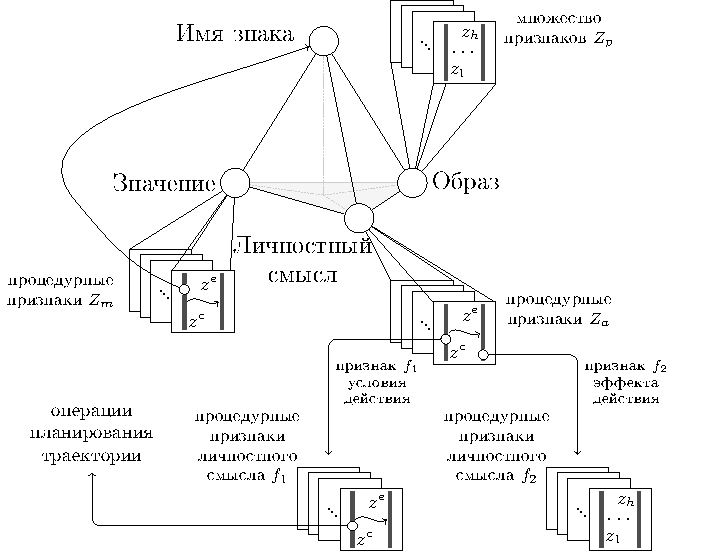
\includegraphics[width=0.7\textwidth]{signs/sign_details_ru}
			\end{column}
		\end{columns}
		\par\bigskip
		Нейрофизиологические данные свидетельствуют в пользу существования такой структуры (Эдельман, Иваницкий, Маунткастл и др.)
		\nocite{*}
		\printbibliography[keyword={nerosign}, resetnumbers=true]
		
	\end{frame}

	\begin{frame}
		\frametitle{Картина мира субъекта деятельности \footnotesize (Осипов, Панов, Чудова)}
		
		\begin{columns}
			\begin{column}{0.55\textwidth}
				\begin{figure}
					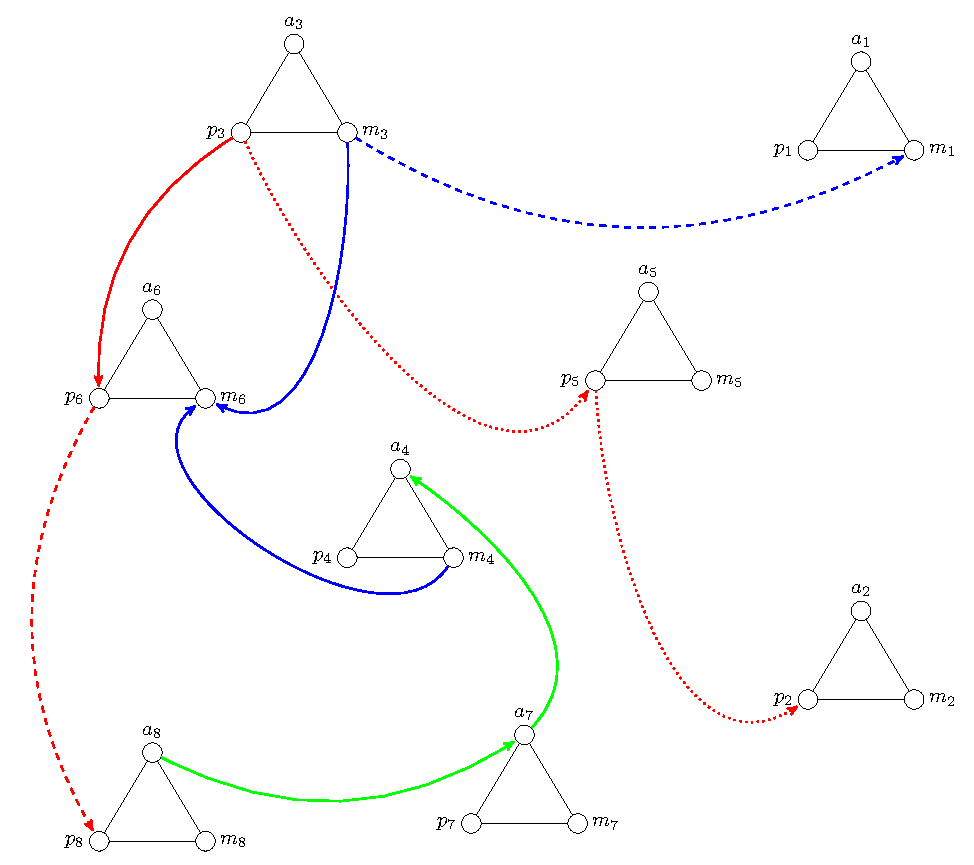
\includegraphics[width=\textwidth]{signs/signs_net}
				\end{figure}
			\end{column}
			\begin{column}{0.45\textwidth}
				\textit{Семиотическая сеть} $H=\langle H_P, H_A, H_M\rangle$, где
				\begin{itemize}
					\item $H_P=\langle2^P,\mathfrak R_P\rangle$ "--- семантическая сеть на множестве образов знаков,
					\item $H_P=\langle2^A,\mathfrak R_A\rangle$ "--- семантическая сеть на множестве значений знаков,
					\item $H_P=\langle2^M,\mathfrak R_M\rangle$ "--- семантическая сеть на множестве личностных смыслов знаков.
				\end{itemize}
			\end{column}
		\end{columns}
	\end{frame}	

	\begin{frame}
		\frametitle{Модель процесса восприятия --- алгоритм $\mathfrak A_{th}$}
		
		\begin{tikzpicture}[overlay,remember picture]
		
		\tikzstyle{z_matrix} = [draw, rectangle, minimum width = 60, minimum height = 60,fill=white];
		
		\onslide<1->{
			\node (meas_fun) at (0.7,0.5) {$\hat f_1,\hat f_2\dots,\hat f_k$};	
		}
		\onslide<2->{
			\node (control_vect) at ($(meas_fun)+(-0.5,1.2)$) {$\hat x^{j+1}$};
			\path[->,thick,red] (control_vect.east)  edge[out = -45, in = 45, right] (meas_fun.north); 
		}
		\onslide<3->{
			\node[z_matrix] (z_1) at ($(meas_fun)+(2.6,-0.5)$) {};
			\node[z_matrix] at ($(z_1)+(0.2,-0.1)$) {};
			\node[z_matrix] at ($(z_1)+(0.4,-0.2)$) {};
			
			\node[z_matrix] at ($(z_1)+(0.9,-0.5)$) {};
			\node[z_matrix] at ($(z_1)+(1.1,-0.6)$) {};
			\node[z_matrix] at ($(z_1)+(1.3,-0.7)$) {};
			
			\path[->,thick,blue] ([xshift=20]meas_fun.south)  edge[out = -90, in = -155, right] ($(z_1)+(-1,-1.2)$);
			\path[->,thick,blue] ([xshift=-25]meas_fun.south)  edge[out = -90, in = -155, right] ($(z_1)+(-0.1,-1.7)$);
			
			\node at ($(z_1)+(-1,1.4)$) {$Z^*$};
			
			\node at ($(z_1)+(0.8,1.4)$) {$Z_1$};
			\node at ($(z_1)+(1.4,1.2)$) {$\ddots$};
			\node at ($(z_1)+(2,0.9)$) {$Z_k$};
		}
		
		\onslide<4->{
			\draw[ultra thick, green!60!black] ($(z_1)+(-0.4,-1.1)$) -- ($(z_1)+(-0.4,0.6)$);
			\draw[ultra thick, green!60!black] ($(z_1)+(0.5,-1.6)$) -- node[right,black] {$z_1^r$} ($(z_1)+(0.5,0.1)$);
			
			\draw[->, thick, green!60!black] ($(z_1)+(-0.1,-3)$) -- node[right,black] {$\bar x(0)$} ($(z_1)+(-0.1,-2)$);
		}
		
		\onslide<5->{
			\node[z_matrix] (z_2) at ($(z_1)+(5,0)$) {};
			\node[z_matrix] at ($(z_2)+(0.2,-0.1)$) {};
			
			\node[z_matrix] at ($(z_2)+(0.9,-0.5)$) {};
			\node[z_matrix] at ($(z_2)+(1.3,-0.7)$) {};
			
			\node at ($(z_2)+(-1,1.4)$) {$Z^*$};
			\node at ($(z_2)+(0.8,1.4)$) {$Z_1$};
			\node at ($(z_2)+(1.4,1.2)$) {$\ddots$};
			\node at ($(z_2)+(2,0.9)$) {$Z_k$};
			
			\draw[->, ultra thick] ($(z_1)+(2.6,-0.6)$) -- node [above] {\scriptsize$\frac{\|\bar z_1^r-\bar x(0)\|}{\|\bar z_1^r\|+\|\bar x(0)\|}$} ($(z_1)+(3.7,-0.6)$);
			
			\draw[ultra thick, dotted, green!60!black] ($(z_2)+(-0.6,-1)$) -- ($(z_2)+(-0.6,0.7)$);
			\draw[ultra thick, dotted, green!60!black] ($(z_2)+(0.5,-1.6)$) -- ($(z_2)+(0.5,0.1)$);
		}
		
		
		\onslide<6->{
			\draw[->, thick, red] ($(z_2)+(0.3,1.4)$) -- node[right,black] {$\bar x^*(0)$} ($(z_2)+(0.3,3)$);
		}
		
		\onslide<7>{
			\draw[<-, thick, red] ($(z_2)+(-0.1,-3)$) -- node[right,black] {$\hat x^j(0)$} ($(z_2)+(-0.1,-2)$);
		}
		
		\onslide<7->{				
			\draw[ultra thick, green!60!black] ($(z_2)+(-0.4,-1)$) -- ($(z_2)+(-0.4,0.7)$);
			\draw[ultra thick, green!60!black] ($(z_2)+(0.7,-1.6)$) -- node[right,black] {$z_2^r$} ($(z_2)+(0.7,0.1)$);	
		}
		\onslide<8->{
			\draw[->, thick, green!60!black] ($(z_2)+(-0.1,-3)$) -- node[right,black] {$\bar x(1)$} ($(z_2)+(-0.1,-2)$);
		}
		
		\onslide<9->{
			\draw[->, ultra thick] ($(z_2)+(2.6,-0.6)$) -- node [above] {\scriptsize$\frac{\|\bar z_1^r-\bar x(1)\|}{\|\bar z_1^r\|+\|\bar x(1)\|}$} ($(z_2)+(3.7,-0.6)$);
		}
		\end{tikzpicture}
	\end{frame}

	\begin{frame}
		\frametitle{Модель процесса обучения \footnotesize (Панов, Петров, Скрынник)}
		
		К основным принципам работы механизма обучения относятся: 
		
		\begin{itemize}
			\item использование иерархии вычислительных узлов с восходящими и нисходящими связями, 
			\item использование Хэббовских правил обучения, 
			\item разделение пространственного и временного группировщиков, 
			\item подавление второстепенной активации для формирования разреженного представления.
		\end{itemize}
		
		Формируемые в результате работы механизма обучения связи задают матрицу предсказания для некоторого выходного признака в модели распознающих автоматов.
		
	\end{frame}
	
	\begin{frame}
		\frametitle{Модель процесса целеполагания \footnotesize (Осипов, Панов)}
		\centering
		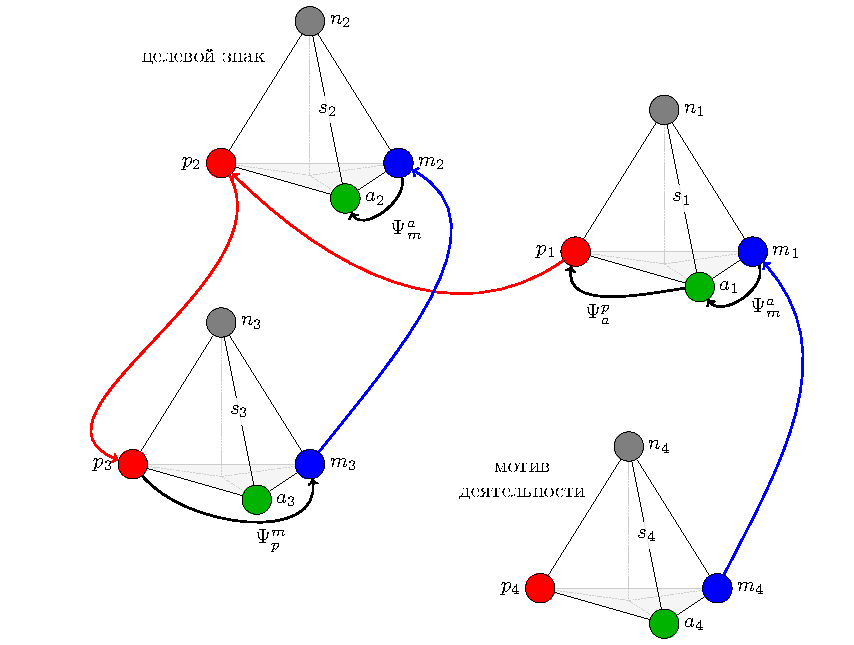
\includegraphics[width=0.7\textwidth]{algo/ru/goal_set_alg_ru}
	\end{frame}	
	
	\begin{frame}
		\frametitle{Модель процесса планирования поведения}
		\centering
		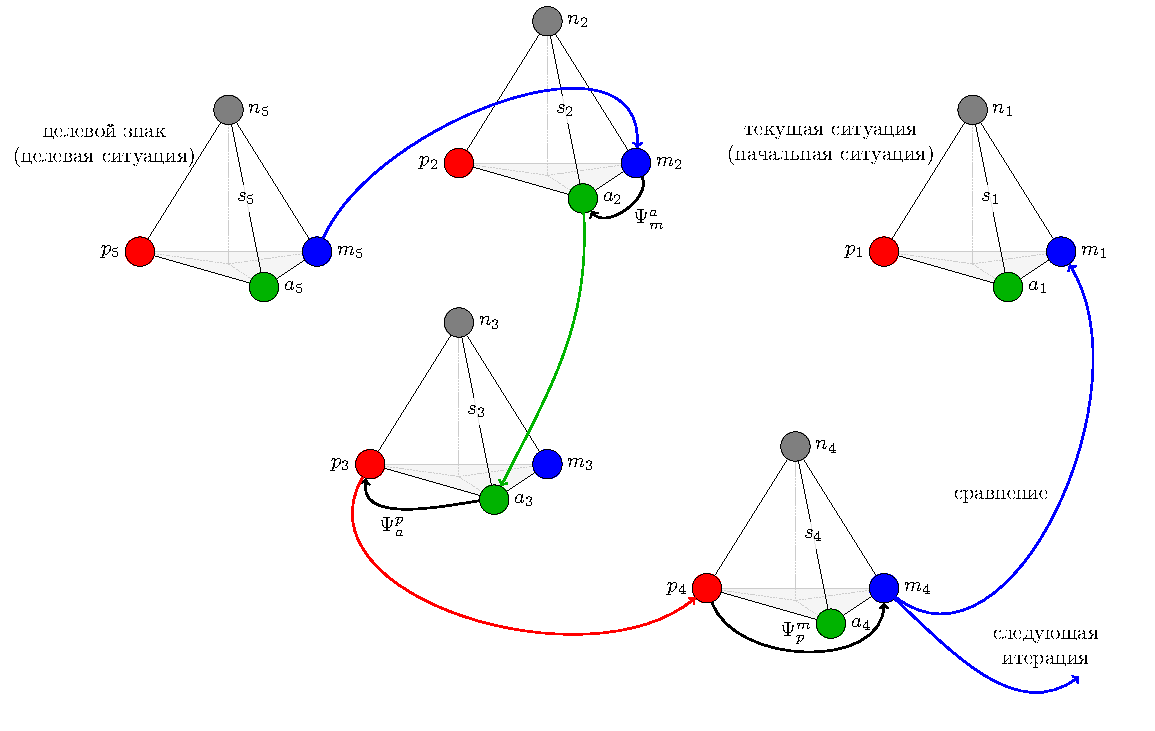
\includegraphics[width=\textwidth]{algo/ru/plan_alg_ru}
	\end{frame}	
		
	\begin{frame}
		\frametitle{Алгоритм планирования поведения}
		
		\begin{columns}
			\begin{column}{0.7\textwidth}
				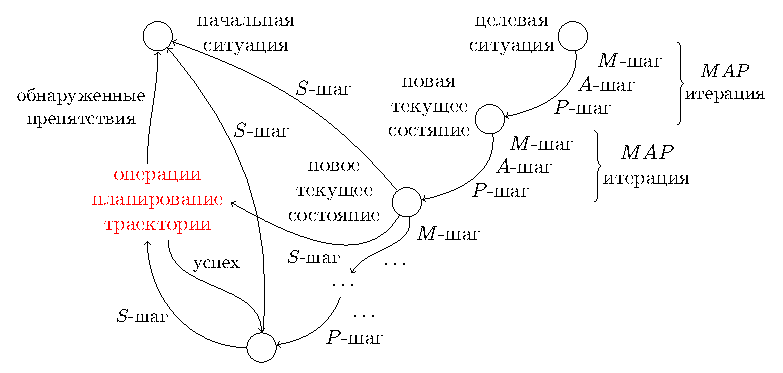
\includegraphics[width=\textwidth]{algo/ru/beh_plan_ru}
			\end{column}
			\begin{column}{0.3\textwidth}
				\tiny
				Процесс планирования начинается с конченой ситуации и стремится достичь начальной ситуации.
				\par\bigskip
				Основные шаги алгоритма (MAP-итерации):
				\begin{itemize}
					\item \textit{M-step} -- поиск применимых действий на сети значений,
					\item \textit{A-step} -- подбор личностных смыслов, соответствующих найденным значениям,
					\item \textit{P-step} -- построение новой текущей ситуации по множеству признаков условий найденных действий,
					\item \textit{S-step} -- отправка сообщения другим участникам коалиции или выполнение найденного действия или активаций иерархии операция вплоть до операций планирования пути.
				\end{itemize}
			\end{column}
		\end{columns}
		\nocite{*}
		\printbibliography[keyword={behplan}, resetnumbers=true]
	\end{frame}	

	\begin{frame}
		\frametitle{Особенности постановки задачи}
		
		Рассматривается случай группового взаимодействия автономных технических объектов (агентов), в котором:
		\begin{itemize}
			\item агенты решают общую задачу (имеют общую цель высшего уровня),
			\item агенты действуют независимо друг от друга (децентрализованное управление), в т.ч. могут ставить индивидуальные подцели и достигать их,
			\item агенты обладают различными характеристиками, как техническими, так и когнитивными, т.е. разными стратегиями поведения,
			\item агенты обладают различными картинами мира,
			\item агенты действуют в меняющейся среде.
		\end{itemize}
		
	\end{frame}
	
	\begin{frame}
		\frametitle{Требования к представлению знаний}
		
		На представление пространственных и временных знаний в задаче согласованного перемещения с такими особенностями налагается ряд ограничений:
		\begin{itemize}
			\item необходимость поддержки некоторого протокола коммуникации, разделение знаний на коммуницируемые и некоммуницируемые (личные),
			\item необходимость выделения компоненты знания, не зависящей от индивидуальных (личных) характеристик агента,
			\item требование к наличию механизма связывания реальных объектов внешней среды и процедур их распознавания с символьным коммуницируемым представлением (symbol grounding problem),
			\item поддержка механизмов пополнения картины мира (обучение и абстрагирование).
		\end{itemize}
	\end{frame}
		
	\begin{frame}
		\frametitle{Задача интеллектуального перемещения \footnotesize (Панов, Яковлев)}
		
		\begin{columns}
			\begin{column}{0.55\textwidth}
				\begin{center}
					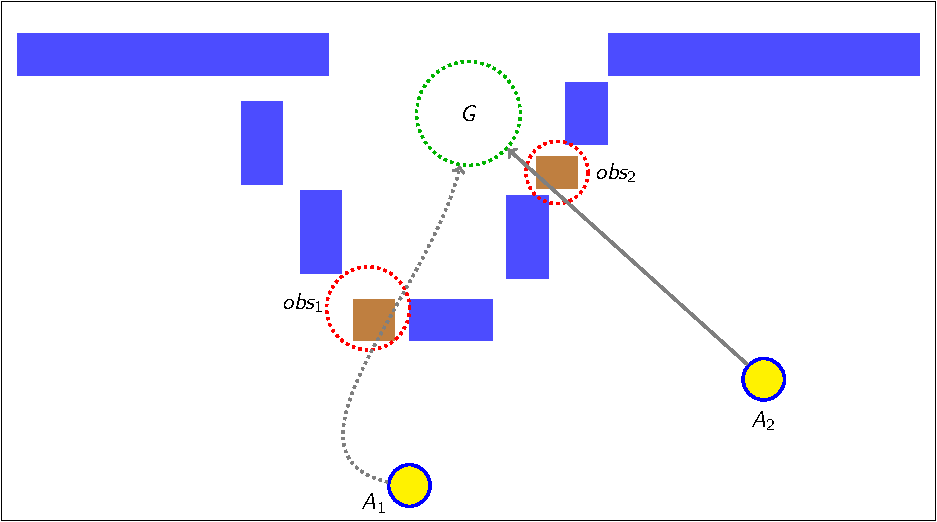
\includegraphics[page=1,width=0.8\textwidth]{examples/slides_colored}
				\end{center}
				\vspace{-7pt}
				\small
				\textbf{Задача}
				
				Целевая область не достижима некоторым агентом самостоятельно (с использованием только методов планирования траектории).
				
				\textbf{Решение}
				
				Агенты должны поддерживать коммуникацию и модифицировать свои собственные планы с учетом коалиционных подзадач.
				
			\end{column}
			\begin{column}{0.45\textwidth}
				Особенности:
				\begin{itemize}
					\item Меняющаяся внешняя среда.
					\item Различные типы препятствий (некоторые могут быть разрушены).
					\item Агенты обладают различной функциональностью.
					\item Общая пространственная цель (ВСЕ агенты должны достичь определенной области на карте).
				\end{itemize}
			
			\end{column}
		\end{columns}
	\end{frame}
	
	\begin{frame}
		\frametitle{Представление пространственных знаний}
		
		\begin{figure}
			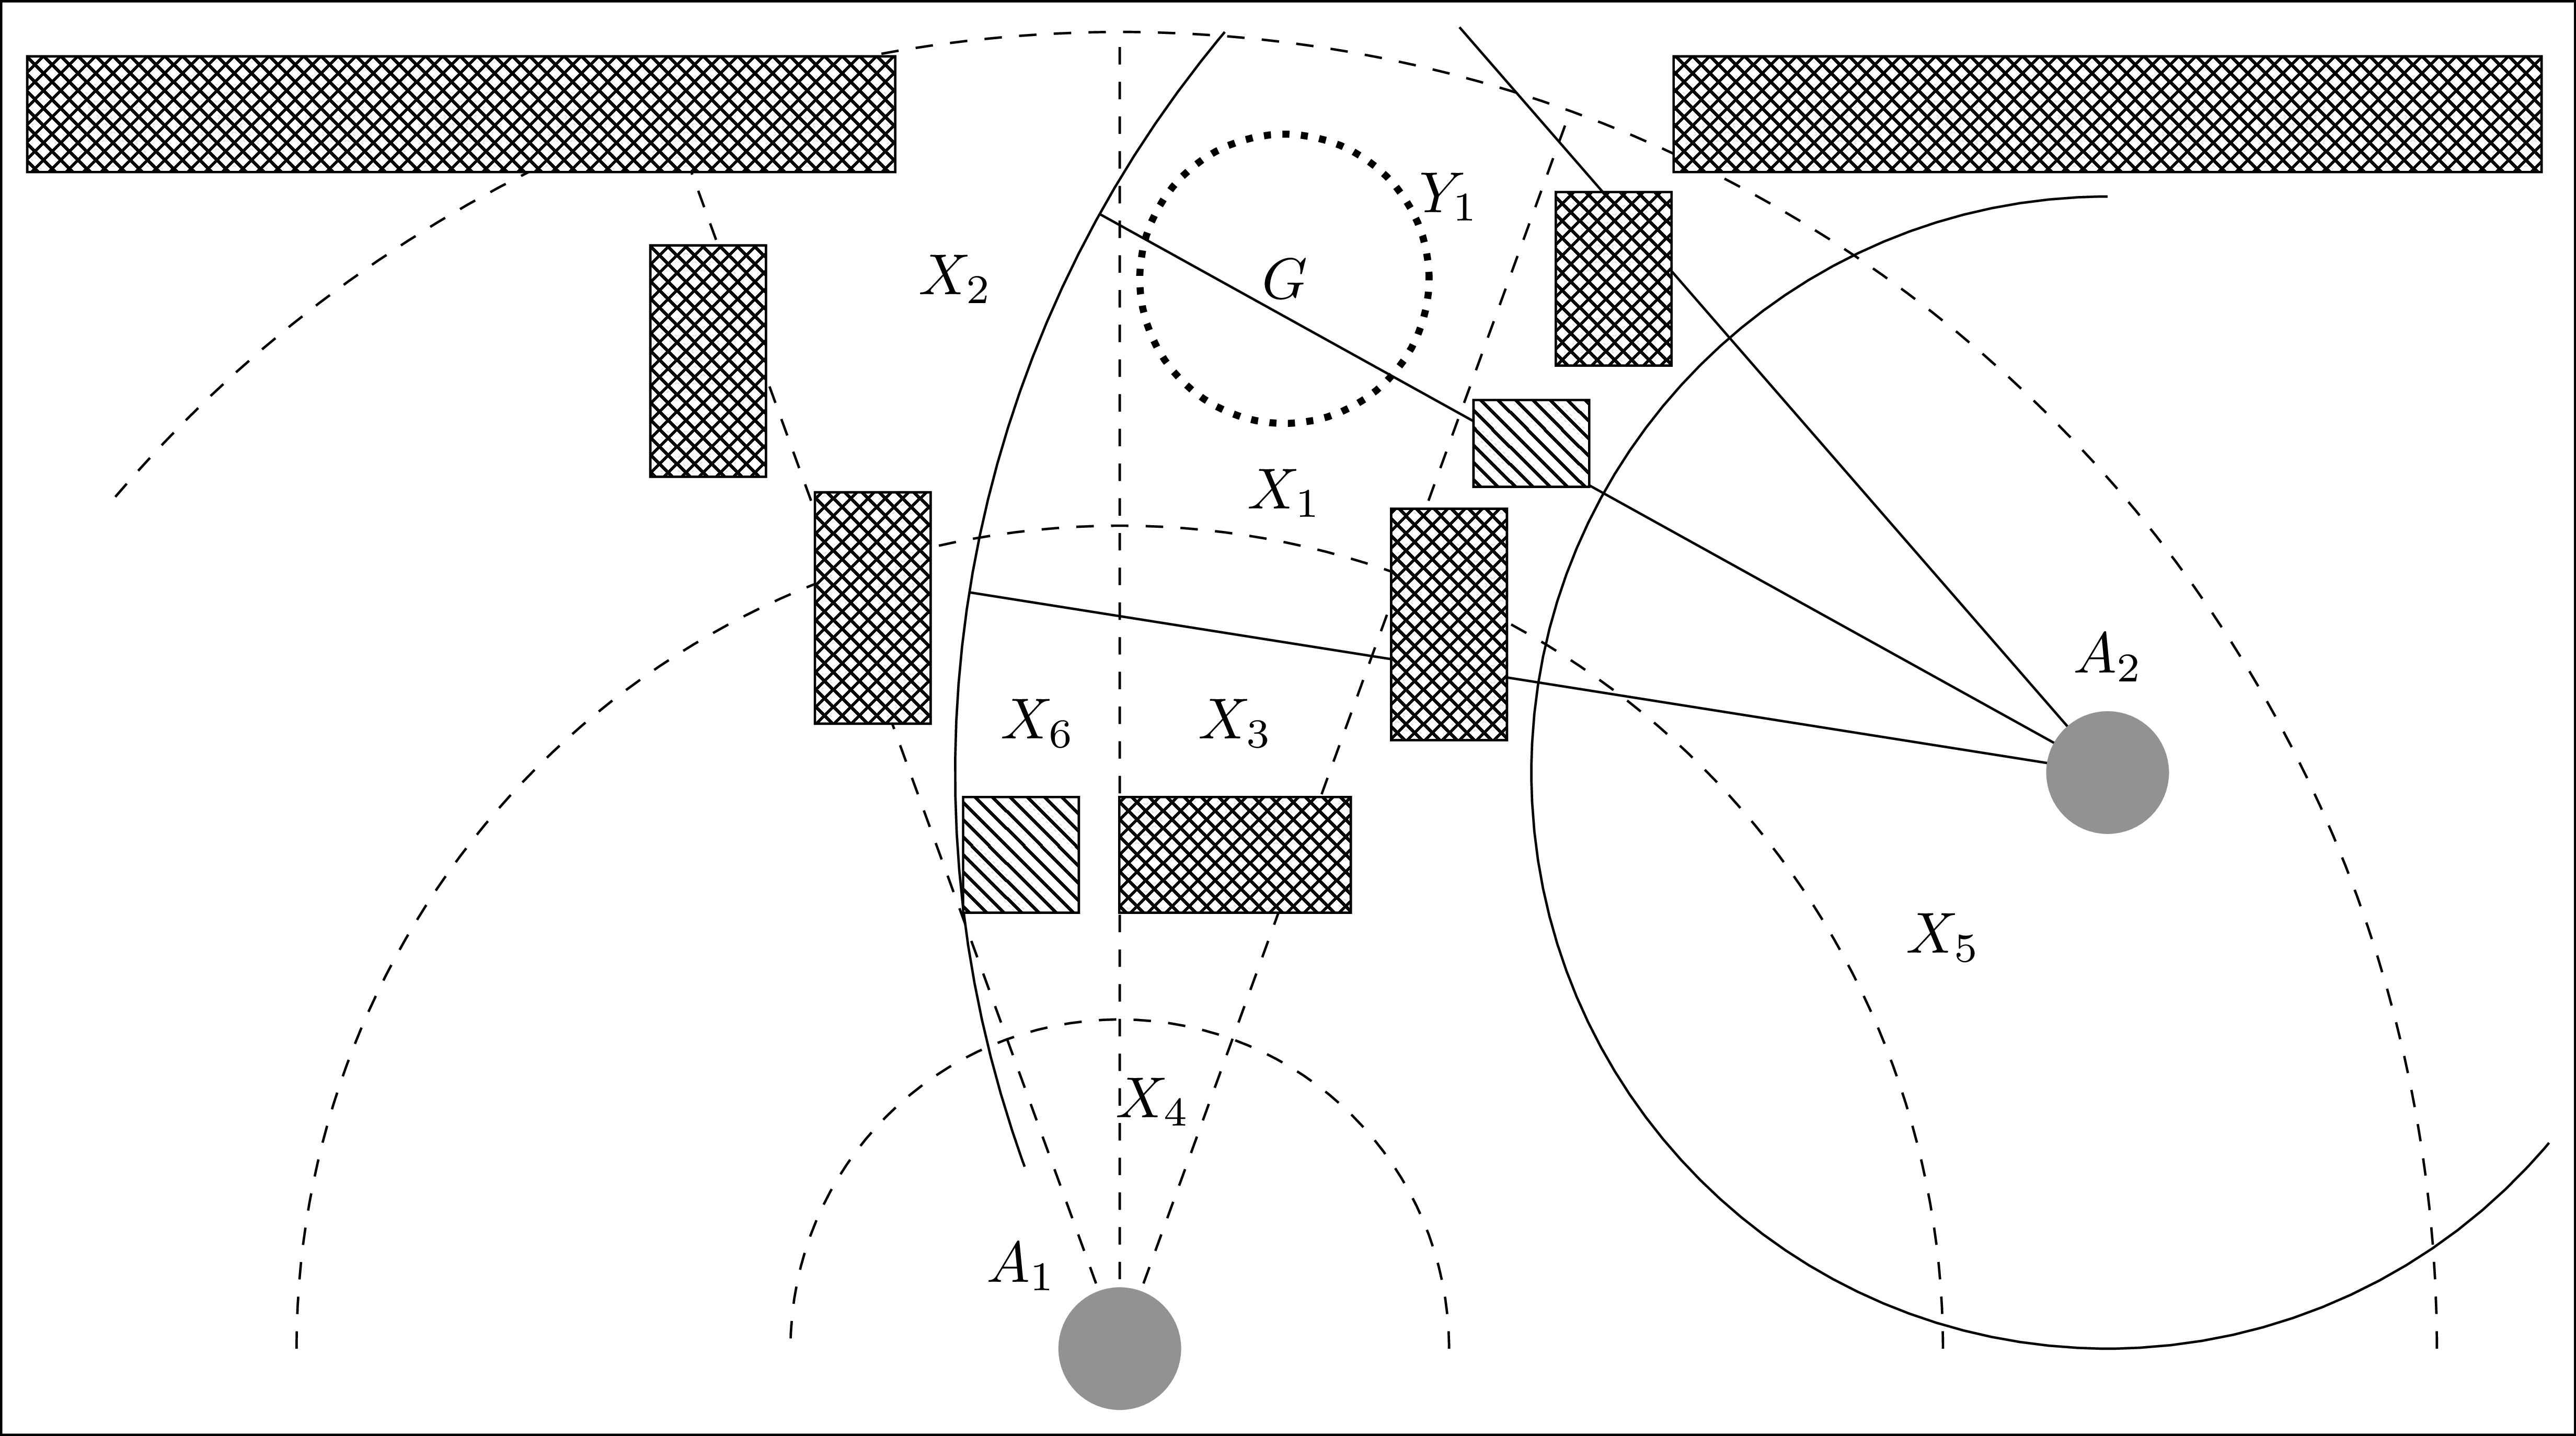
\includegraphics[width=\textwidth]{examples/rita_ex_proc.png}
		\end{figure}
	\end{frame}
	
	\begin{frame}
		\frametitle{Представление действий по перемещению}
		
		Действия по перемещению "--- знаки $s_t$ (признаки $f_t$, $t$ "--- тип перемещения), которым соответствуют матрицы предсказания типа $Z_t$, состоящие из трёх столбцов 
		\[
		z_1=(l_x, I), z_2=(l_y, d_u, E), z_3=(l_y, I, t_v)
		\]
		,где 
		\begin{itemize}
			\item $l_x$, $l_y$ "--- признаки, соответствующие категории расстояния в пространственной логике  (например, вплотную, близко, далеко и др.), 
			\item $d_u$ "--- признак, соответствующий категории направления в пространственной логике (например, впереди, слева и др.), 
			\item $t_v$ "--- признак, соответствующий категории времени во временной логике (например, скоро, в будущем и др.),
			\item $I$ "--- признак присутствия самого агента, 
			\item $E$ "--- признак отсутствия препятствия.
		\end{itemize}
	\end{frame}	
	
	\begin{frame}
		\frametitle{Распределение ролей при решении задачи}
		\begin{center}
			\scalebox{0.7}{
				\animategraphics{12}{examples/slides_colored}{}{}			
			}
		\end{center}
	\end{frame}
	
	\begin{frame}
		\frametitle{Пример по перемещению}
		
		\begin{center}
			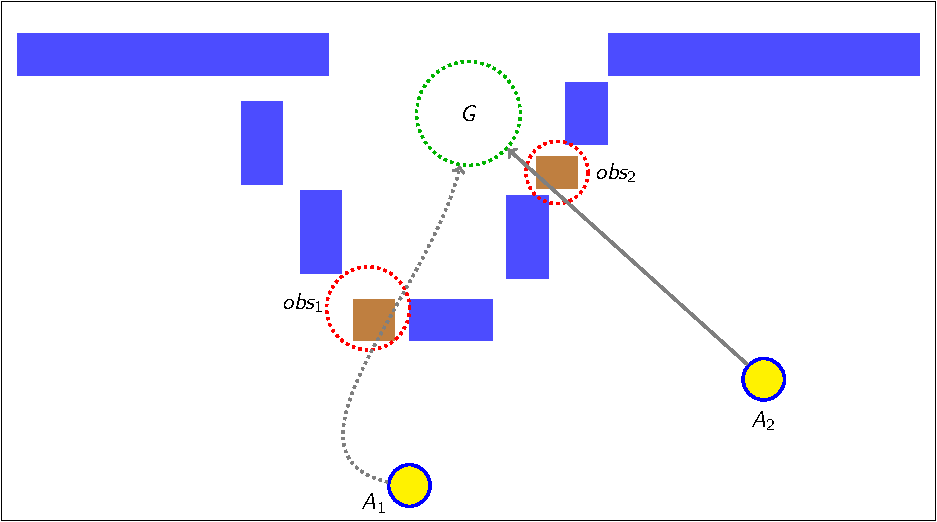
\includegraphics[page=1,width=0.85\textwidth]{examples/slides_colored}
		\end{center}
		\par\bigskip
		Актуализированные знаки агента $A_1$: ``область $X_6$'', ``далеко'', ``перемещение 1'' $\rightarrow$ \color{red} операции планирования траектории.
	\end{frame}
	
	\begin{frame}
		\frametitle{Пример по перемещению}
		
		\begin{center}
			\includegraphics[page=31,width=0.85\textwidth]{examples/slides_colored}
		\end{center}
		\par\bigskip
	Актуализированные знаки агента $A_1$: ``препятствие 1'', ``рядом'', ``область $X_6$''.
	\end{frame}
	
	\begin{frame}
		\frametitle{Пример по перемещению}
		
		\begin{center}
			\includegraphics[page=42,width=0.85\textwidth]{examples/slides_colored}
		\end{center}
		\par\bigskip
		Актуализированные знаки агента $A_1$: ``отправить сообщение'', ``агент $A_2$''.
	\end{frame}
	
	\begin{frame}
		\frametitle{Пример по перемещению}
		
		\begin{center}
			\includegraphics[page=58,width=0.85\textwidth]{examples/slides_colored}
		\end{center}
		\par\bigskip
		Актуализированные знаки агента $A_2$: ``область $Y_3$'', ``далеко'', ``перемещение 2'' $\rightarrow$ \color{red} операции планирования траектории.
	\end{frame}
	
	\begin{frame}
		\frametitle{Пример по перемещению}
		
		\begin{center}
			\includegraphics[page=95,width=0.85\textwidth]{examples/slides_colored}
		\end{center}
		\par\bigskip
		Актуализированные знаки агента $A_2$: ``область $Y_1$'', ``рядом'', ``препятствие 1'', ``разрушить''.
	\end{frame}
	
	\begin{frame}
		\frametitle{Пример по перемещению}
		
		\begin{center}
			\includegraphics[page=116,width=0.85\textwidth]{examples/slides_colored}
		\end{center}
		\par\bigskip
		Актуализированные знаки агента $A_1$ and $A_2$: ``далеко'', ``перемещение 3'' $\rightarrow$ \color{red} операции планирования траектории.
	\end{frame}
	
	\begin{frame}
		\frametitle{Пример по перемещению}
		
		\begin{center}
			\includegraphics[page=171,width=0.85\textwidth]{examples/slides_colored}
		\end{center}
		\par\bigskip
		Актуализированные знаки агента $A_1$ и $A_2$: целевое состояние (``область $G$'').
	\end{frame}
			
	\begin{frame}
		\frametitle{Применение для решения интеллектуальных задач}
		
		\begin{itemize}
			\item Моделирование внимания,
			\item образование нового знания (концепта),
			\item планирование поведения,
			\item построение картины мира субъекта на основе текстов,
			\item генерация сообщений на основе картин мира определенного типа (виртуальные ассистенты),
			\item построение многоуровневых архитектур управления.
		\end{itemize}
	\end{frame}

	\begin{frame}
		\frametitle{Некоторые публикации}
		\renewcommand*{\bibfont}{\tiny}
		\nocite{*}
		\printbibliography
	\end{frame}

	\begin{frame}
		\centering
		\Huge
		Спасибо за внимание!
		\normalsize
		\par\bigskip
		\par\bigskip
		ФИЦ ИУ РАН, лаб. <<Динамические интеллектуальные системы>>, pan@isa.ru
	\end{frame}

	\begin{frame}
		\frametitle{Кратко о себе}
		\scriptsize
		\begin{columns}
			\begin{column}{0.85\textwidth}
				\textbf{Панов Александр Игоревич, к. ф.-м. н.}
				\begin{itemize}
					%					\item Научный сотрудник лаборатории <<Динамические интеллектуальные системы>> Института системного анализа Федерального исследовательского центра <<Информатика и управление>> Российской академии наук.
					%					\item Научный сотрудник и старший преподаватель в Высшей школе экономики.
					%					\item Ассистент в Московском физико-техническом институте.
					\item Член редколлегии журнала Biologically Inspired Cognitive Architectures (BICA Journal).
					\item Член Российской ассоциации искусственного интеллекта (РААИ).
					\item Член Сообщества биологически инспирированных когнитивных архитектур (BICA Society).
					\item Организатор Международной	школы по биологически инспирированным когнитивным архитектурам (Fierces on BICA, Москва) и Международной конференции по биологически инспирированным когнитивным архитектурам (BICA-2016, Нью-Йорк).
					\item Член рабочей группы <<Нейронет>> Национальной технологической инициативы.
					\item Руководитель проектов РФФИ мол\_а и мол\_а\_дк.
				\end{itemize}
			\end{column}
			
			\begin{column}{0.15\textwidth}
				\centering
				
\includegraphics[width=\textwidth]{advert/ras.png}
				\vspace{7pt}
				
\includegraphics[width=0.7\textwidth]{advert/isa.png}
				\vspace{7pt}
				
\includegraphics[width=0.5\textwidth]{advert/raai.png}
				\vspace{7pt}
				
\includegraphics[width=0.5\textwidth]{advert/hse.png}
				\vspace{7pt}
				
\includegraphics[width=\textwidth]{advert/mipt.jpg}
				\vspace{7pt}
				
\includegraphics[width=\textwidth]{advert/bica2016.png}
				\vspace{7pt}
				
\includegraphics[width=0.7\textwidth]{advert/nti.jpg}
			\end{column}
			
		\end{columns}
	\end{frame}
	
	\begin{frame}
		\frametitle{Научные интересы}
		
		\begin{itemize}
			\item \textit{Когнитивное компьютерное моделирование}: планирование поведения, модели внимания, восприятия, принятия решений и обучения, знаковые системы.
			\item \textit{Многоагентные системы}: образование коалиций, распределение ролей в коллективе, целеполагание.
			\item \textit{Анализ данных}: выявление причинно-следственных связей, анализ психологических и медицинских данных.
			\item \textit{Распознавание изображение}: выявление объектов на сложных сценах, рекуррентные и глубокие нейронные сети.
			\item \textit{Системы управления}: управление поведением, многоуровневые архитектуры, робототехника.
		\end{itemize}
	\end{frame}
	
	\begin{frame}
		\frametitle{Подгруппа когнитивного компьютерного моделирования}
		\begin{columns}
			\begin{column}{0.65\textwidth}
				\begin{itemize}
					\item Осипов Геннадий Семенович, д.ф.-м.н.
					\item Чудова Наталья Владимировна, к.псих.н.
					\item Кузнецова Юлия Михайловна, к.псих.н.
					\item Панов Александр, к.ф.-м.н.
					\item Петров Александр
					\item Киселев Глеб, асп. ИСА РАН
					\item Скрыник Алексей, студ. РГАТУ
					\item Кудинов Антон, студ. ВШЭ
					\item Филин Дмитрий, студ. ВШЭ
				\end{itemize}
			\end{column}
			\begin{column}{0.35\textwidth}
				\begin{tikzpicture}
				\node at (-0.2,-1.7) {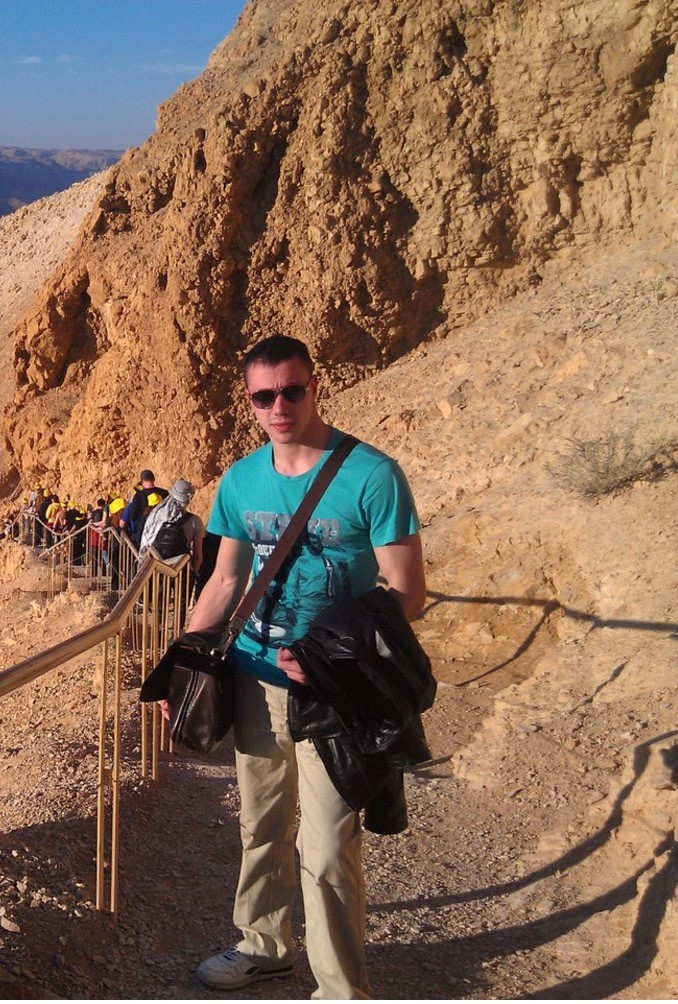
\includegraphics[width=0.7\textwidth]{misc/kiselev}};
				\node at (-2.3,2) {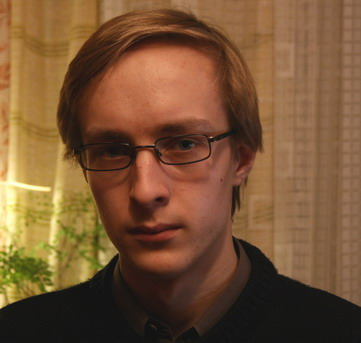
\includegraphics[width=0.6\textwidth]{misc/petrov}};
				\node at (-0.3,1) {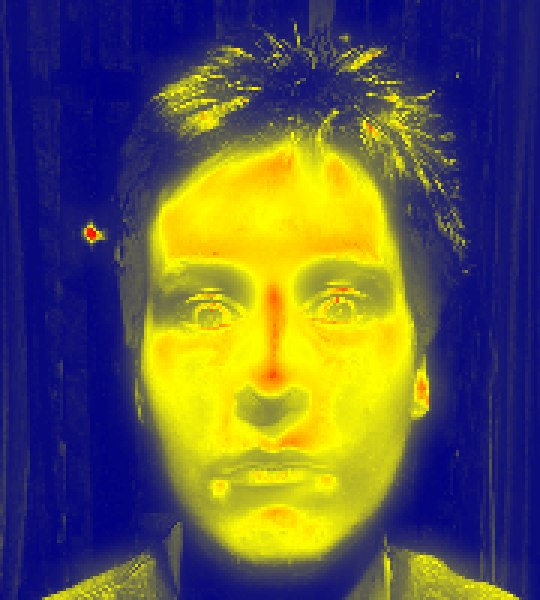
\includegraphics[width=0.5\textwidth]{misc/kudinov}};					
				\node at (-2.8,-1) {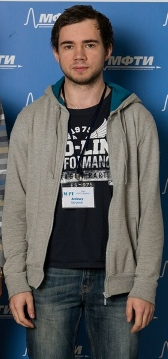
\includegraphics[width=0.5\textwidth]{misc/skrynnik}};
				\end{tikzpicture}
			\end{column}
		\end{columns}		
	\end{frame}		
														
%	\begin{frame}
%		\frametitle{Цели курса}
%		
%		\begin{columns}
%			\begin{column}{0.5\textwidth}
%				
%			\end{column}
%			\begin{column}{0.5\textwidth}
%				\begin{figure}
%					
\includegraphics[width=\textwidth]{logo}
%				\end{figure}
%			\end{column}
%		\end{columns}
%	\end{frame}
	%	\begin{frame}
	%		\frametitle{Цели курса}
	%		
	%		\begin{itemize}
	%			\item
	%		\end{itemize}
	%	\end{frame}
	
\end{document}
	
	
